\documentclass{article} % For LaTeX2e
\usepackage{nips15submit_e,times}
\usepackage[colorlinks,linkcolor=red]{hyperref}
\usepackage{url}
\usepackage{amsmath}
\usepackage{graphicx}
\usepackage{float}
\usepackage{bm}
\usepackage{amssymb}
%\documentstyle[nips14submit_09,times,art10]{article} % For LaTeX 2.09


\title{CS499 Homework 8 (First Draft)}


\author{
	Intersteller\thanks{ Use footnote for providing further information
		about author (webpage, alternative address)---\emph{not} for acknowledging
		funding agencies.}
	Department of Computer Science
	Cranberry-Lemon University
	Pittsburgh, PA 15213
}

% The \author macro works with any number of authors. There are two commands
% used to separate the names and addresses of multiple authors: \And and \AND.
%
% Using \And between authors leaves it to \LaTeX{} to determine where to break
% the lines. Using \AND forces a linebreak at that point. So, if \LaTeX{}
% puts 3 of 4 authors names on the first line, and the last on the second
% line, try using \AND instead of \And before the third author name.

\newcommand{\fix}{\marginpar{FIX}}
\newcommand{\new}{\marginpar{NEW}}

%\nipsfinalcopy % Uncomment for camera-ready version

\begin{document}

	\maketitle
	\textbf{Exercise 8.1}\par
	\quad 1.\par
  	\begin{figure}[H]
  	\centering
  	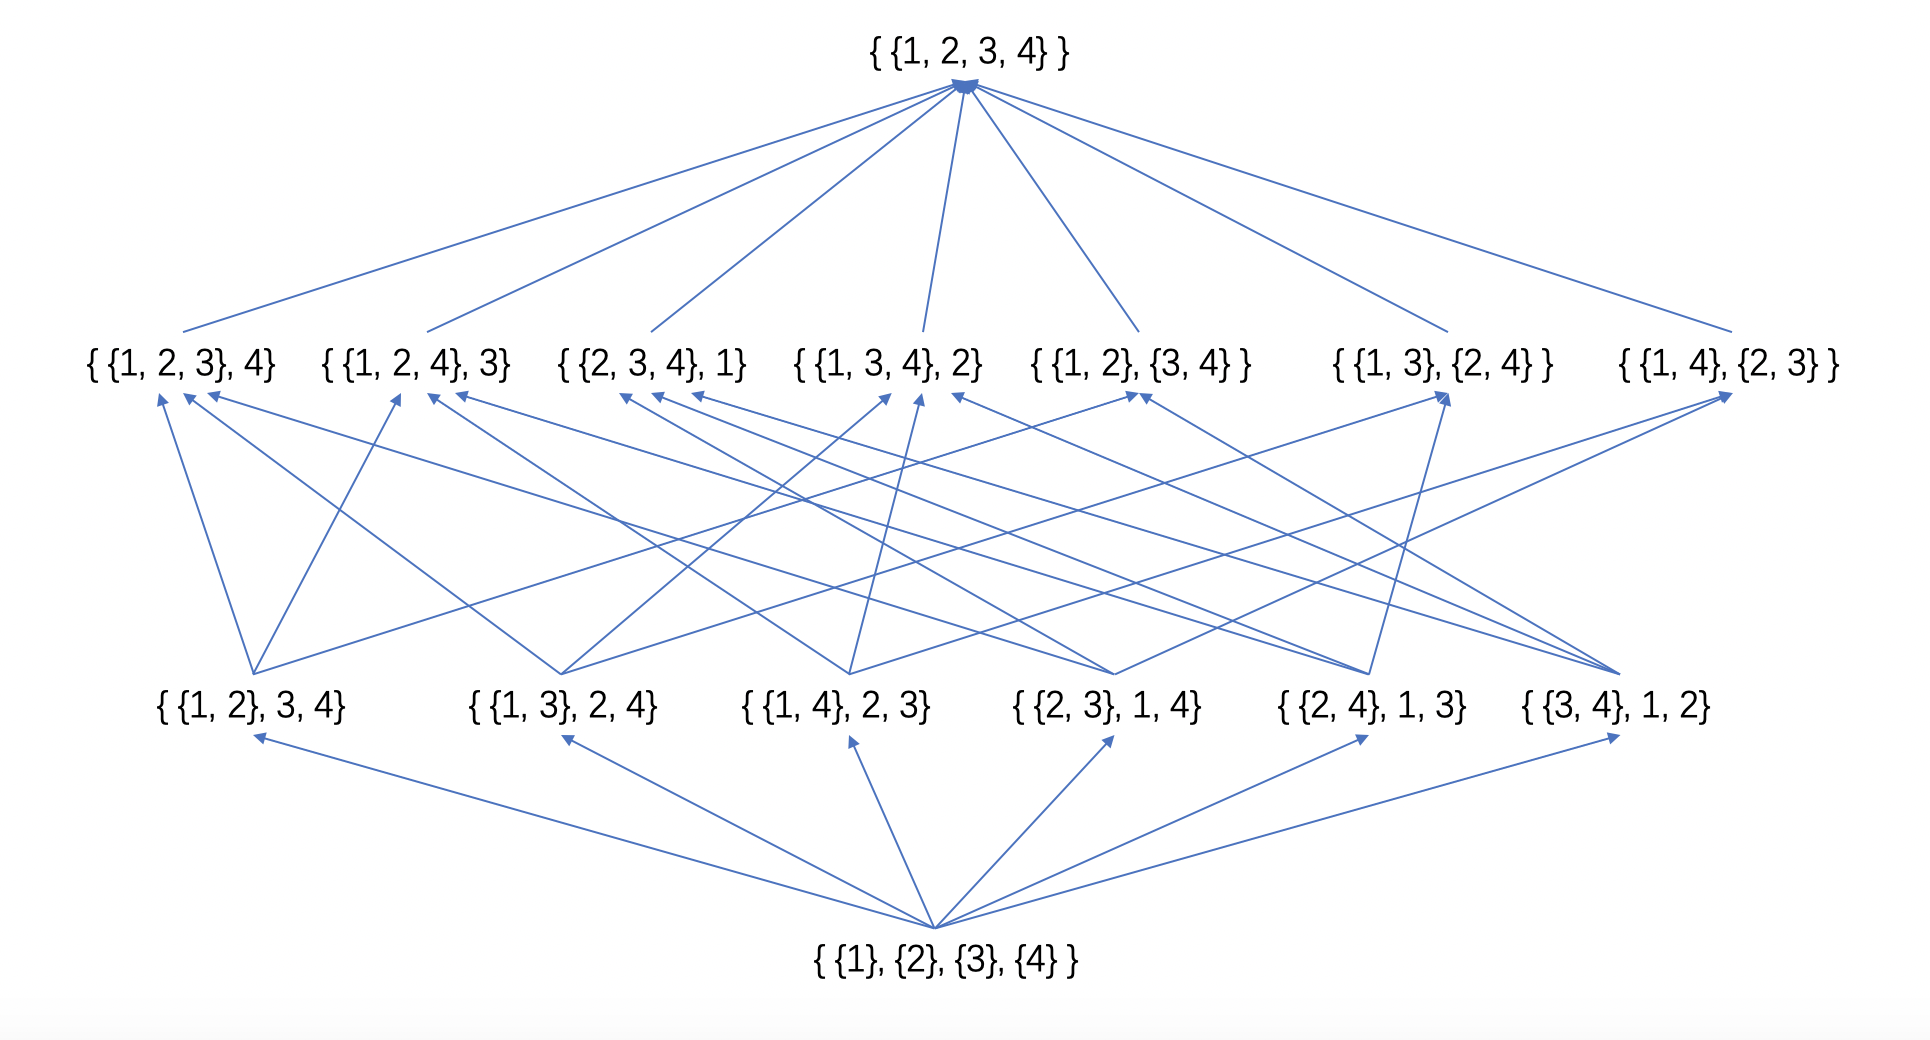
\includegraphics[scale=0.5]{8_1.png}
  	\caption{}
  	\label{}
  	\end{figure}
	\quad 2. The size of the largest chain is $4$.\par
	 \quad 3. The size of the largest antichain is $7$.\par 
	\textbf{Exercise 8.4}\par
	We assume that $(\mathbb{N}_{0}^{n},\leq)$ has an infinite antichain $T$. Obviously, $T \subseteq  (\mathbb{N}_{0}^{n},\leq)$. 
	According to \textbf{exercise 8.3}, we get $T$ contains an infinite chain, which contradicts $T$ is an infinite antichain. 
	Thus $(\mathbb{N}_{0}^{n},\leq)$ has no infinite antichain.\par
	\textbf{Exercise 8.5}\par
	$n=2$\par
	 \begin{figure}[H]
  	\centering
  	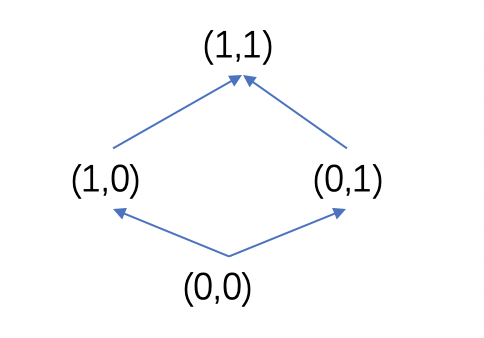
\includegraphics[scale=0.5]{8_5_1.png}
  	\caption{}
  	\label{}
  	\end{figure}
	$n=3$\par
	\begin{figure}[H]
  	\centering
  	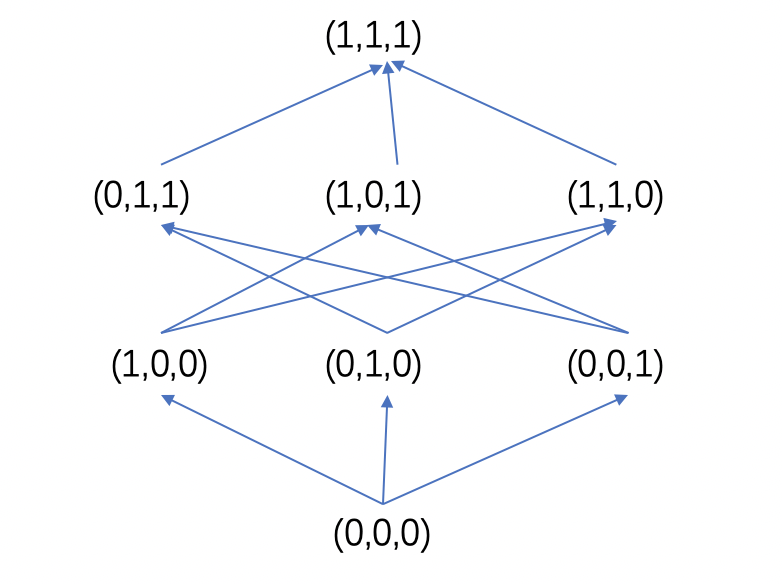
\includegraphics[scale=0.5]{8_5_2.png}
  	\caption{}
  	\label{}
  	\end{figure}
	\textbf{Exercise 8.6}\par
	Maximum is $(\underbrace{1,1,1,\cdots,1}_{n})$\par
	Minimum is $(\underbrace{0,0,0,\cdots,0}_{n})$\par
	Maximal is  $(\underbrace{1,1,1,\cdots,1}_{n})$\par
	Minimal is $(\underbrace{0,0,0,\cdots,0}_{n})$\par
	\textbf{Exercise 8.7}\par
	We construct the Hasse diagrams like \textbf{Exercise 8.5}. 
	The first layer is an element with $n$ one. The second layer is $n$ elements with $n-1$ one.
	The third layer is $\binom{2}{n}$ elements with $n-2$ one......The $k$ layer is $\binom{k-1}{n}$ elements with $n+1-k$ one, where $1\leq k\leq n+1$.\par
	Obviously elements in the same layer is antichain, since elements in chain must have different numbers of one and in the same layer the number of one is equivalent.
	Thus it has $n+1$ antichain partition.\par
	According to Mirsky's Theorem, max size of chain$=$min size of antichain partition. It means max size of chain must less than or equal to the size of each antichain partition. 
	Thus the longest chain of ${\{0,1\}}^n$ $\leq n+1$. Since we get $n+1$ antichain partition in above Hasse diagrams, then the longest chain of ${\{0,1\}}^n$ is $n+1$.\par 
	

	


	\textbf{Question:}\par
	


\end{document}
	

